\paragraph{QuizziPedia::Front-End::Views::ProfileManagementView}
\begin{figure} [ht]
	\centering
	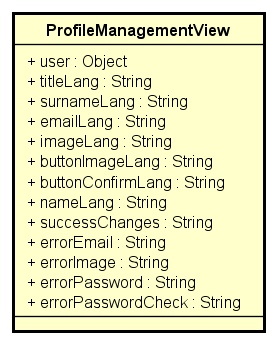
\includegraphics[scale=0.80]{UML/Classi/Front-End/QuizziPedia_Front-end_Views_ProfileManagementView.png}
	\caption{QuizziPedia::Front-End::Views::ProfileManagementView}
\end{figure} \FloatBarrier
\begin{itemize}
	\item \textbf{Descrizione}: view contenente i dati personali che un utente può modificare dopo essersi registrato al sistema;
	\item \textbf{Utilizzo}: permette all'utente di modificare tutti i campi elencati, tranne l'username, e di rendere persistenti tali modifiche se sono accettate dal sistema;
	\item \textbf{Relazioni con altre classi}:
	\begin{itemize}
		\item \textit{IN} \texttt{ProfileManagementModelView}: classe di tipo modelview la cui istanzazione è contenuta all'interno della variabile di ambiente \$scope di \texttt{Angular.js}. All'interno di essa sono presenti le variabili e i metodi necessari per il \textit{Two-Way Data-Binding\ped{G}} tra la view \texttt{ProfileManagementView} e il controller \texttt{ProfileManagementController};
		\item \textit{IN} \texttt{LangModel}: rappresenta il modello delle informazioni per la giusta traduzione dell'applicazione.
	\end{itemize}
	\item \textbf{Attributi}:
	\begin{itemize}
		\item \texttt{+ user: Object} \\ Campo dati contenente i seguenti attributi: \texttt{name: String}, \texttt{surname: String}, \texttt{email: String}, \texttt{password: String} e \texttt{passwordCheck: String};
		\item \texttt{+ imageObject: Object} \\ Oggetto contenente i seguenti attributi: \texttt{+ imageUrl: String}, \texttt{+ image: Object};
		\item \texttt{+ titleLangProfileManagement: String} \\ Attributo che viene utilizzato per visualizzare la giusta traduzione del titolo della pagina, in italiano o in inglese;
		\item \texttt{+ nameLangProfileManagement: String} \\ Attributo che viene utilizzato per visualizzare la giusta traduzione della \textit{label\ped{G}} per l'inserimento del nome, in italiano o in inglese;
		\item \texttt{+ surnameLangProfileManagement: String} \\ Attributo che viene utilizzato per visualizzare la giusta traduzione della \textit{label\ped{G}} per l'inserimento del cognome, in italiano o in inglese;
		\item \texttt{+ emailLangProfileManagement: String} \\ Attributo che viene utilizzato per visualizzare la giusta traduzione della \textit{label\ped{G}} per l'inserimento della posta elettronica, in italiano o in inglese;
		\item \texttt{+ imageLangProfileManagement: String} \\ Attributo che viene utilizzato per visualizzare la giusta traduzione della \textit{label\ped{G}} per l'inserimento dell'immagine, in italiano o in inglese;
		\item \texttt{+ buttonImageLangProfileManagement: String} \\ Attributo che viene utilizzato per visualizzare la giusta traduzione della \textit{label\ped{G}} per il bottone di caricamento immagine, in italiano o in inglese;
		\item \texttt{+ buttonConfirmLangProfileManagement: String} \\ Attributo che viene utilizzato per visualizzare la giusta traduzione della \textit{label\ped{G}} per il bottone di conferma, in italiano o in inglese;
		\item \texttt{+ successChanges: String} \\ Attributo che visualizza un messaggio di conferma avvenute modifiche;
		\item \texttt{+ errorEmail: String} \\ Attributo che visualizza un eventuale messaggio di errore nell'inserimento della email;
		\item \texttt{+ errorPassword: String} \\ Attributo che visualizza un eventuale messaggio di errore nell'inserimento della password;
		\item \texttt{+ errorPasswordCheck: String} \\ Attributo che visualizza un eventuale messaggio di errore nell'inserimento della password di conferma.
	\end{itemize}
\end{itemize}